\section{Opgaver}
%%
\subsection*{Differentialregning}
%%
\begin{opgave}{Hastighed og postion}
	\begin{figure}[h!]
		\centering
		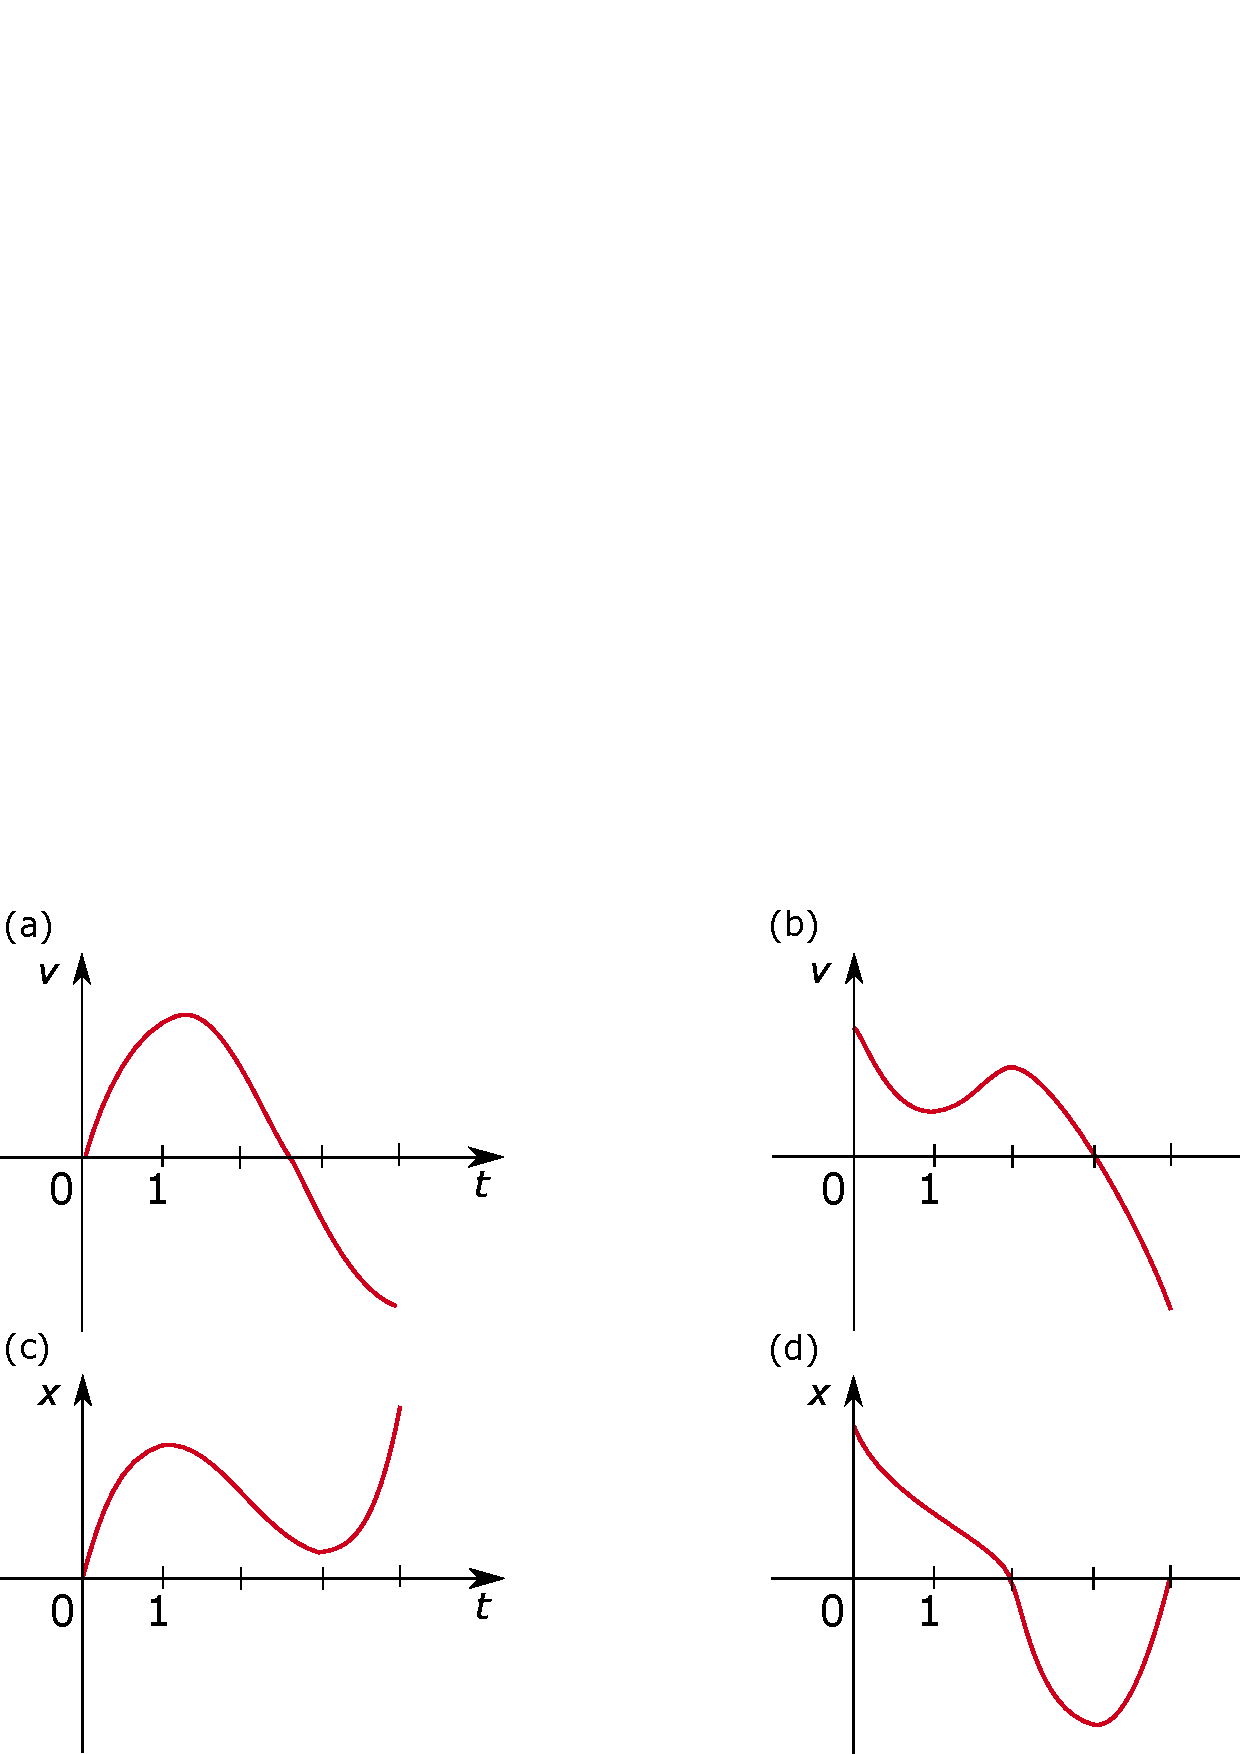
\includegraphics[width=0.47\textwidth]{opg/figurer/vx_grafer.png}
		\caption{Hastighed og position som funktion af tiden.}
		\label{fig:vx_grafer}
	\end{figure}
	\opg Figur \ref{fig:vx_grafer} (a) og (b) viser hastigheden af to objekter som funktion af tiden i sekunder. Hvornår sætter de to objekter hastigheden op, og hvornår sætter de hastigheden ned? Forklar dit svar.
	\opg Figur \ref{fig:vx_grafer} (c) og (d) viser positionen af to objekter $x$ som funktion af tiden i sekunder. Hvornår sætter de to objekter hastigheden op, og hvornår sætter de hastigheden ned? Forklar dit svar.
\end{opgave}
%%
%%
\begin{opgave}{Afledede og dobbeltafledede}
Find den afledede og dobbeltafledede med hensyn til $x$ for følgende funktioner:
\opg $f(x) = x^2 + 4x.$
\opg $f(x) = \frac{1}{x} + \frac{1}{x^2}.$
\opg $f(x) = \cos(x).$
\opg $f(x) = \ln(x).$
\opg $f(x) = x \sin(x).$
\opg $f(x) = \frac{1}{x} \ln(x).$
\end{opgave}
%%
%%
\begin{opgave}{Sammensatte funktioner}
Skriv følgende udtryk som en sammensat funktion $f(g(x))$ (altså skal du identificere den indre funktion $g(x)$ og den ydre funktion $f(g)$). Beregn derefter $\dv{f}{x}$.\\ 
\opg $f(x) = \sin (4x).$
\opg $f(x) = \sqrt{2x}.$
\opg $f(x) = \sqrt{4x+5}.$
\opg $f(x) = \sin(e^x).$
\opg $f(x) =  \ln \left( \cos x \right).$
\end{opgave}
%%
\subsection*{Integralregning}
%%
\begin{opgave}{Integraler og arealer under funktioner}
I matematikafsnittet i kompendiet nævnes det, at når man regner et bestemt integral
\begin{equation*}
\int^a_b{f(x)}\dd{x},
\end{equation*}
så svare det til arealet under grafen for $f(x)$ i intervallet $[a,b]$ på $x$-aksen. Brug dette faktum til at diskutere den fysiske forståelse af følgende udsagn.
\opg Hvis man integrerer en hastighed $v(t)$ ift. tiden $t$, så får man en position $x(t)$.
\opg Hvis man integrerer en acceleration $a(t)$ ift. tiden $t$, så får man en hastighed $v(t)$. \\
\end{opgave}
%%
%%
\begin{opgave}{Ubestemte integraler}
	Udregn det ubestemte integral af følgende funktioner:
	\opg $f(x) = x^3$.
	\opg $f(x) = x^2 + 4x$.
	\opg $f(x) = x^2 + \frac{1}{x^2}$.
	\opg $f(x) = \cos (x)$.
	\opg $f(x) = \frac{1}{x}$.
\end{opgave}
%%
\begin{opgave}{Størrelsen af en port}
    En tømmer er blevet hyret til at lave tre porte.
    Toppen af hver port kan beskrives med en af de følgende funktioner
    \begin{align*}
        f(x)&=1-x^2,\\
        g(x)&=2-\frac{e^x+e^{-x}}{2},\\
        h(x) &= 1-\abs{x}.        
    \end{align*}
    Alle portene er i intervallet $[-1/2,1/2]$.
    \opg Opstil bestemte integraler til at udregne arealet af de tre porte.
    \opg Hvilken port er størst?
    \opg Hvilken er mindst?
\end{opgave}
%%
\begin{opgave}{Ubestemte højereordensintegraler}
    Udregn følgende ubestemte højereordensintegraler. Sæt alle integrationskonstanter til nul.
    \opg $\iint ye^{-x}\dd{x}\dd{y}.$
    \opg $\iint y\cos(xy)\dd{x}\dd{y}.$
    \opg $\iiint (x^2+y^2)z\dd{x}z\dd{y}\dd{z}.$
    \opg $\iiint \sin(x)\sin(y)\sin(z)\dd{x}\dd{y}\dd{z}.$
\end{opgave}
%%
%%
%\begin{opgave}{Bestemte højere ordens integraler}
    %Udregn følgende bestemte højere ordens integraler
    %\opg $\int_0^1\int^0_{-\ln(2)} ye^{-x}\dd{x}\dd{y}$
    %\opg $\int_0^1\int_0^\pi y\cos(xy)\dd{x}\dd{y}$
    %\opg $\int_{-1}^1\int_{0}^{x}\int_{-1}^1 (x^2+y^2)z\dd{x}z\dd{y}\dd{z}$
    %\opg $\int_0^\pi\int_0^\pi\int_0^\pi \sin(x)\sin(y)\sin(z)\dd{x}\dd{y}\dd{z}$
%\end{opgave}
%%
%%
%\begin{opgave}{Lige og ulige funktioner} \label{opg:lige/ulige}
%En funktion, så som $f(x) = x^2$, der opfylder kravet, $f(x) = f(-x)$, kaldes en lige funktion. En funktion, som $f(x) = x$, der opfylder det lignende krav, $f(x)=-f(-x)$, kaldes for en ulige funktion.
%Det vil sige, at en lige funktion er uændret, hvis man spejler den i $y$-aksen, mens en ulige funktion skifter fortegn ved den samme spejling.
%Bemærk at de fleste funktioner er hverken lige eller ulige, og unikt er funktionen $f(x) = 0$ både lige og ulige.
%Afgør om følgende funktioner er lige eller ulige.
%\opg $\sin(x)$.
%\opg $e^{x^2}$.
%\opg $\cos(x)$.
%\end{opgave}
%%
%%
%\begin{opgave}{Integraler af lige og ulige funktioner.}
%Vi vil her finde nogle meget praktiske regneregler for integraler af lige og ulige funktioner, der er defineret i opgave \thechapter,\ref{opg:lige/ulige}, over et symmetrisk interval.
%Lad $f_l(x)$ være en lige funktion og $f_u(x)$ være en ulige funktion.
%Antag derudover at integralerne
%$$
%\int_0^a f_l(x)\dd{x}   \quad \text{og} \quad \int_0^a f_u(x)\dd{x}
%$$
%er kendte.
%\opg Vis at
%$$
%\int_{-a}^{a} f_l(x)\dd{x} = 2\int_0^a f_l(x) \, .
%$$
%\opg Vis at
%$$%\int_{-a}^{a} f_u(x)\dd{x} = 0 \, .
%$$
%\opg Brug dette til at løse integralet: $$\int_{-1}^1 {x^2\cos(x)\sin(x)+x^2-xe^{x^2}}\dd{x}$$
%\end{opgave}
%%
%%
%\begin{opgave}{Et spøjst integral}
    %Udregn
    %\opg $\int_0^{\pi} \cos(x)\dd{x}$
    %\opg $\int_\pi^{2\pi} \cos(x)\dd{x}$
    %\opg $\int_0^{2\pi} \cos(x)\dd{x}$
    %\opg $\int_0^{\pi/2} \cos(x)\dd{x}$
    %\opg $\int_{-8\pi}^{32\pi} \cos(x)\dd{x}$
    %\opg $\int_{-8\pi}^{32\pi} \cos[2019](x)\dd{x}$
    %\opg $\int_{-2019\pi}^{2019\pi} %\cos[2019](x)\dd{x}$
%\end{opgave}
%%
\subsection*{Differentialligninger}
%%
\begin{opgave}{Hvornår er det en løsning?}
	I denne opgave skal vi finde ud af, hvornår nogle forskellige funktioner er løsninger til de givne differentialligninger. Sagt med andre ord skal vi finde de specifikke talværdier for alle de konstanter, der indgår i funktionerne, således at funktionerne løser deres respektive differentialligningerne. Bemærk at der kan være mere end 1 værdi.
	\opg For hvilke værdier af $k$ løser funktionen
	\begin{align*}
	f(x) = \cos(kx)
	\end{align*}
	differentialligningen
	\begin{align*}
	4 \dv[2]{f(x)}{x} = - 25f(x) \, .
	\end{align*}
	\opg Tjek for de værdier af $k$ I fandt i 1), at funktionen $g(x) = A \sin (kx) + B \cos (kx)$ også løser differentialligningen
	\begin{align*}
	4 \dv[2]{g(x)}{x} = -25 g(x) \, .
	\end{align*}
	\opg For hvilke værdier af $r$ løser funktionen
	\begin{align*}
	h(x) = e^{rx}
	\end{align*}
	differentialligningen
	\begin{align*}
	2 \dv[2]{h(x)}{x} + \dv{h(x)}{x} - h(x) = 0 \, .
	\end{align*}
	\opg Lad $r_1$ og $r_2$ være de konstanter du fandt i \textbf{3)}. Tjek at funktionen $k (x) = ae^{r_1x} + be^{r_2x} $ også løser differentialligningen
	\begin{align*}
	2 \dv[2]{k(x)}{x} + \dv{k(x)}{x} - k(x) = 0 \, .
	\end{align*}
\end{opgave}
%%
%%
\begin{opgave}{Generelle 1. ordens differentialligninger}
I denne opgave skal du også vise, at nogle forskellige funktioner er løsninger til de givne differentialligninger. Denne gang er funktionerne og differentialligningerne dog skrevet op på en mere generel form, dvs. at de kan indeholde arbitrære konstanter.
\opg Vis at alle funktioner på formen
\begin{align*}
	h(x) = \frac{1}{x + A} 
\end{align*}
løser differentialligningen
\begin{align*}
	\dv{h}{x} = - h(x)^2 \; .
\end{align*}
\opg Vis at alle funktioner på formen
\begin{align*}
	k(x) = \left( c - x^2 \right)^{-1/2}
\end{align*}
løser differentialligningen
\begin{align*}
	\dv{k}{x} = x k(x)^3 \; .
\end{align*}
\opg Vis at alle funktioner på formen
\begin{align*}
	g(x) = \frac{\ln (x) + C}{x}
\end{align*}
løser differentialligningen
\begin{align*}
	x^2 \dv{g}{x} + xg(x) = 1 \; .
\end{align*} 
\opg Vis at alle funktioner på formen
\begin{align*}
	f(x) = \frac{1 + ce^x}{1-ce^x}
\end{align*}
løser differentialligningen
\begin{align*}
	\dv{f}{x} = \frac{1}{2} \left( f(x)^2 - 1 \right) \; .
\end{align*} 
\end{opgave}
%%
%%
%\begin{opgave}{Brugbare differentialligninger}
    %Bestem hvilken funktion f(t), der opfylder de følgende differentialligninger
   %\opg $\dv{f(t)}{t} = c \cdot f(t)$, hvor c er en arbitrær konstant, $c \neq 0$
   %\opg ${\dv{f(t)}{t}} = \frac{1}{2\cdot f(t)} $
   %\opg Vis at $f(t)=t^{2/3}$ er en løsning til differentialligningen 
   %$\dv{f(t)}{t} = \frac{2}{3\sqrt{f(t)}}$
%\end{opgave}
%%
%%
%\begin{opgave}{Dejlige andenordens differentialligninger, der er værd at kende}
    %Løs de følgende differentialligninger
    %\opg $\dv[2]{f(x)}{x}=0$
    %\opg $\dv[2]{g(x)}{x}=k$
    %\opg $\dv[2]{h(x)}{x} + h(x) = 0 $
    %\opg $\dv[2]{f(x)}{x} + \dv{f(x)}{x} = 0 $
    %\opg $\dv[2]{g(x)}{x} + \dv{g(x)}{x} = k $
    %\opg $\dv[2]{h(x)}{x} + \dv{h(x)}{x} + h(x) = 0 $
%\end{opgave}
%%
\subsection*{Logaritmer}
%%
\begin{opgave}{Logaritmeopgaver I}
    Find værdien af de følgende udtryk
    \opg $\log_{4}(8).$
    \opg $\log_{1/9}\left(\sqrt{27}\right).$
    \opg $\ln(e^{2/3}).$
    \opg $\ln(\frac{e^5}{e^3}).$
\end{opgave}
%%
%%
\begin{opgave}{Logaritmeopgaver II}
    Løs for den ukendte variabel
    \opg $\log_{b}(16) = 4/3.$
    \opg $\ln(x) = -1.$
    \opg $\log_{2}(1/x)=\frac{1}{5}.$
\end{opgave}
%%
%%
%\begin{opgave}{Logaritmeapproximationer}
%Brug approximationerne $\log_{10}(2) = 0,3010$ og $\log_{10}(3)= 0,4771$ til at udregne værdien af de følgende udtryk
    %\opg $\log_{10}(24)$
    %\opg $\log_{10}(5)$
    %\opg $\log_{10}(4^{\frac{1}{3}})$
%\end{opgave}
%%
%%
\begin{opgave}{En ekstra logaritmeregneregel}
    Ud fra de tre logaritmeregneregler, \eqref{mat:log}, vis at
    $$
    \frac{\log(a)}{b}=\log(a^{-b}).
    $$
\end{opgave}